% !TeX spellcheck = de_DE
\documentclass[ngerman,hyperref={pdfpagelabels=false}]{beamer}

% -----------------------------------------------------------------------------

\graphicspath{{images/}}

% -----------------------------------------------------------------------------

\usetheme{KIT}

\setbeamercovered{transparent}
%\setbeamertemplate{enumerate items}[ball]

\newenvironment<>{KITtestblock}[2][]
{\begin{KITcolblock}<#1>{#2}{KITblack15}{KITblack50}}
{\end{KITcolblock}}

\usepackage[ngerman,english]{babel}
\usepackage[utf8]{inputenc}
\usepackage[TS1,T1]{fontenc}
\usepackage{array}
\usepackage{multicol}
\usepackage[absolute,overlay]{textpos}
\usepackage{beamerKITdefs}
\usepackage{amsfonts}


\pdfpageattr {/Group << /S /Transparency /I true /CS /DeviceRGB>>}	%required to prevent color shifting withd transparent images


\title{A Linear-Time Algorithm For Finding Tree-Decompositions Of Small Treewidth}
\subtitle{Maximilian F. Göckel -- \textit{uzkns@student.kit.edu}}

\author[Maximilian Göckel]{Maximilian F. Göckel}
\institute{Institut für Theoretische Informatik - Proseminar Algorithmen für NP-schwere Probleme}

\TitleImage[width=\titleimagewd,height=\titleimageht]{titel}

\KITinstitute{Institut f\"ur Theoretische Informatik}
\KITfaculty{Proseminar NP-schwere Probleme}

% -----------------------------------------------------------------------------

\begin{document}
\setlength\textheight{7cm} %required for correct vertical alignment, if [t] is not used as documentclass parameter


% title frame
\begin{frame}
  \maketitle
\end{frame}



%Voraussetzungen
\begin{frame}
\frametitle{Tree-decomposition}
\framesubtitle{Definition}
\ \\ 
Eine Baumzerteilung eines Graphen $G=(V,E)$ ist ein Tupel $(X, T)$ wo $T =(I, F)$ ein Baum ist und $X = \{ X_i | i \in I \}$ eine Familie von Teilmengen von $V$ wobei jedes $X_i$ einen Knoten in $T$ darstellt. \\
\ \\
\begin{enumerate}
	\item $\bigcup\limits_{i \in I} X_i = V$
	\item $\forall (v,w) \in E: \exists i \in I: v,w \in X_i$
	\item $\forall w \in X_i, X_j : $ Jedes $X_k$ im Pfad zwischen $X_i, X_j$ enthält $w$
\end{enumerate}
\end{frame}


%Beispiel
\begin{frame}
\frametitle{Tree-decomposition}
\framesubtitle{Veranschaulichung}

\begin{figure}[htbp] 
	\centering
	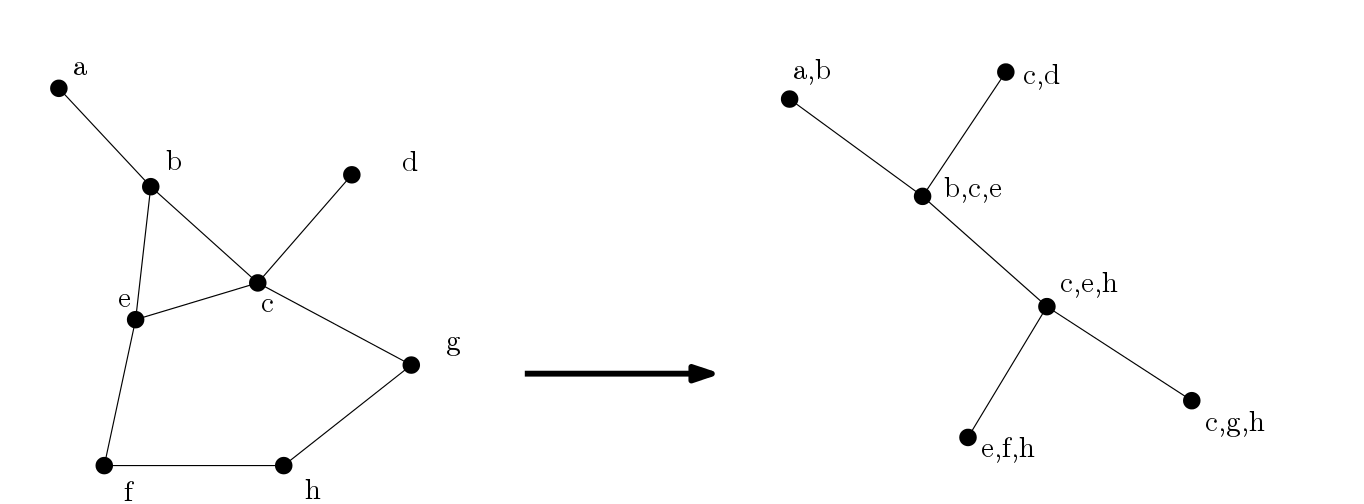
\includegraphics[width=0.7\textwidth]{tree_2.png}
	\caption{1}
	\label{fig:Bild1}
\end{figure}

\end{frame}


%\begin{frame}
%\frametitle{Tree-decomposition: Beispiel}
%
%\begin{figure}[htbp] 
%	\centering
%	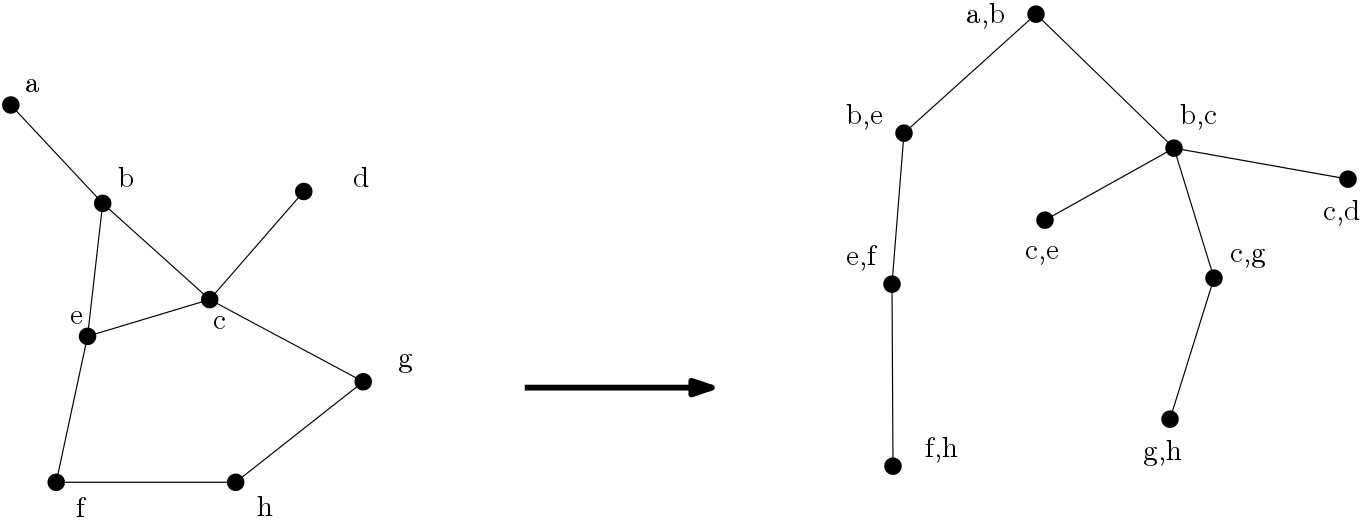
\includegraphics[width=0.7\textwidth]{tree_1.png}
%	\caption{2}
%	\label{fig:Bild1}
%\end{figure}
%
%\end{frame}


%treewidth
\begin{frame}
\frametitle{Treewidth}
\framesubtitle{Definition}

Jede Baumzerteilung hat eine "Baumweite" (treewidth). \\

\begin{itemize}
	\item Baumweite einer Zerteilung: ${\max}( {|X_i|}_{i \in I} - 1)$ ("Zerteilungsweite")
	\item Baumweite eines Graphen: Minimale Zerteilungsweite aller Zerteilungen
\end{itemize}

\end{frame}


%k trees
\begin{frame}
\frametitle{k-Trees}
\framesubtitle{Definition}

Die folgenden Aussagen zu $k$-Bäumen sind äquivalent:
%Quelle: http://www.ii.uib.no/~pinar/chordal.pdf
\begin{enumerate}
	\item $G = (V,E)$ ist ein $k$-Baum
	\item $G$ ist verbunden und hat eine $k$-Clique, aber keine $(k+2)$-Clique und
	\begin{itemize}
		\item Jeder minimale Seperator von $G$ ist eine $k$-Clique oder
		\item $\forall$ nicht-adjazenten Knotenpaare $x,y \in V$ $\exists$ $k$ Wege $x \rightarrow y$
	\end{itemize} 
	\item $G$ ist verbunden,  $|E| = k|V|- \frac{1}{2}k(k+1)$ und jeder minimale Seperator von $G$ ist eine $k$-Clique
	\item $G$ hat Knoten $v$ mit 3 Eigenschaften:
	\begin{itemize}
		\item deg($v$) = $k$ und
		\item Nachbarknoten von $v$ formen eine $k$-Clique und
		\item $G \ v$ ist $k$-Baum
	\end{itemize}
\end{enumerate}
\ \\
Jeder komplette Graph mit $k$ Knoten ist damit auch ein $k$-Baum.

\end{frame}



%k trees
\begin{frame}
\frametitle{k-Trees}
\framesubtitle{Erstellung}
Andersherum: Ein $k$-Baum-Graph $G$ mit $n \geq k$ Knoten kann aus einem $k$-Baum-Graph $H$ mit $n-1$ Knoten wie folgt erstellt werden: \\

\begin{itemize}
	\item Zu $H$ einen Knoten $u$ hinzufügen ($|V|=(n-1) \rightarrow |V|=n$)
	\item Knoten $u$ mit Knoten $v_1, ... , v_k$ verbinden
\end{itemize}

\ \\
Damit wird Aussage $4$ erfüllt.

\end{frame}


%partial k-trees
\begin{frame}
\frametitle{Partial k-Trees}
\framesubtitle{Definition}

Graph $G=(V,E)$ ist partieller $k$-Baum $\Leftrightarrow$ \\

\begin{itemize}
	\item $G$ ist Teilgraph eines $k$-Baumes
	\item $G$ hat Baumweite max. $k$ %+Beweis?
\end{itemize}
\end{frame}


%Anwendungen Baumzerteilungen
\begin{frame}
\frametitle{Baumzerteilung}
\framesubtitle{Anwendungen}

\begin{itemize}
	\item Maximum-Weight Independent Set in Linearzeit lösbar
	\item Hohe Baumweite $\Leftrightarrow$ Hohe Komplexität in der Systemanalyse
	\item %TODO fu berlin bioinformatik
	\item %TODO planare graphen
\end{itemize}
\end{frame}


\begin{frame}
\frametitle{Knotentypen}
\framesubtitle{Simplizial, freundlich, low- und highdegree}
Ein Knoten $v$ ist ... \\
\begin{itemize}
	\item ... "von niedrigem Grad" wenn deg($v$) $\leq d$
	\begin{itemize}
		\item $d = 2k^3 \cdot (k+1) \cdot (4k^2 +12k + 16)$
		\item Analog: Hoher Grad $\Leftrightarrow$ deg($v$) $> d$
		\item Auch "low-deg.-" und "high-deg.-Knoten" genannt
	\end{itemize}
	\item ... "Freundlich" wenn er low-deg. und adjazent zu einem weiteren low-deg.-Knoten ist
	\item ... "Simplizial" wenn alle Nachbarn in einer Clique sind
	\item ... "I-Simplizial" wenn simp. in $G'$ und deg($v$)$\leq k$ in $G$
\end{itemize}
\end{frame}



\begin{frame}
\frametitle{Verbesserter Graph $G'$}
\framesubtitle{Erstellung und Eigenschaften}

$G'=(V,E')$ ist $G=(V,E)$ mit Kanten $(v,w) \in E' \forall v,w \in V$ sodass $v,w$ min. $k+1$ gem. Nachbarn mit Grad max. $k$ haben. \\
\ \\
\textcolor{cyan}{LEMMA 4.1.}: tw($G$)$\leq k \Leftrightarrow$ tw($G'$)$\leq k$. \\
Außerdem ist jede $k$-Zerteilung von $G$ auch eine $k$-Zerteilung von $G'$ und umgekehrt.

\end{frame}



\begin{frame}
\frametitle{Maximum Matching $M \subseteq E$}

$M \subseteq E$ ist Maxmimum Matching in $G=(V,E) \Leftrightarrow$ Keine 2 Kanten aus $M$ haben gemeinsamen Endknoten und $|M|$ maximal \\
\ \\
Ein Maximal Matching kann in $O(|V|)$ gefunden werden, wenn die Baumweite durch ein $k$ gebunden ist. \\ %LEMMA 2.3.

\end{frame}

\begin{frame}
\frametitle{Anzahl an Friendly-Knoten in $G$}
\textcolor{cyan}{LEMMA 4.2.}: $G$ hat Baumweite max. $k \Rightarrow$ 
1 von 2 muss min. gelten:
\begin{itemize}
	\item $G$ hat min. $\frac{|V|}{4k^2+12k+16} =: \lambda$ Friendly-Knoten
	\item $G'$ hat min. $\frac{1}{8k^2+24k+32}\cdot|V|$ I-simp.-Knoten
\end{itemize}
\ \\
Algorithmus hat eine Fallunterscheidung ab $\lambda$ Friendly-Knoten.


\end{frame}

\begin{frame}
\frametitle{Algorithmus}
\framesubtitle{Fall: Min. $\lambda$ Friendly-Knoten}
\begin{enumerate}
	\item Maximum-Matching $M \subseteq E$ finden
	\item Jede Kante in $M$ kontrahieren um Graphen $\widetilde{G}$ zu erhalten
	\item Wenn Baumweite von $\widetilde{G} > k \Rightarrow$ \textcolor{red}{STOP} 
	\item Kompletten Algorithmus auf $\widetilde{G}$ ausführen um Baumzerteilung $(Y,T)$ von $\widetilde{G}$ auszugeben
	\item Mit \textcolor{cyan}{LEMMA 3.3.} Zerteilung $(X,T)$ aus $(Y,T)$ erstellen %Weite 2k+1
	\item Mit \textcolor{cyan}{THEOREM 2.4.} prüfen ob Weite von $G > k$ ist $\Rightarrow$ \textcolor{red}{STOP}
	\item Zerteilung von G errechnen und ausgeben
	 
\end{enumerate}
\end{frame}

















\end{document}
